During the laboratory session two types of estimation methods were used; one \textit{failure count reliability model} called \textit{The Goel-Okumoto model }and one \textit{time between failure model} called \textit{The Jelinski-Moranda model}. 

\subsection{The Goel-Okumoto model}
Non-homogeneous Poisson process models, NHPP, have turned out to be fairly accurate in describing hardware reliability problems. 

The Goel-Okumoto model assumes that the failure process i modeled by an NHPP model under the following conditions:
\begin{itemize}
\item	The cumulative number of faults detected at time t follows a Poisson distribution.
\item	All faults are independent and have the same chance of being detected.
\item 	All detected faults are removed immediately and no new faults are introduced.
\end{itemize}

\noindent The model defines the expected number of faults found at time t by the mean value function:

$$m(t) = a(1 - e^{-bt})$$

\noindent where $a=$ total number of faults in the program and $b=$ constant of proportionality. The shape of this function is shown in Figure~\ref{goelokumoto} below.

\begin{figure}[htb!]
\centering
	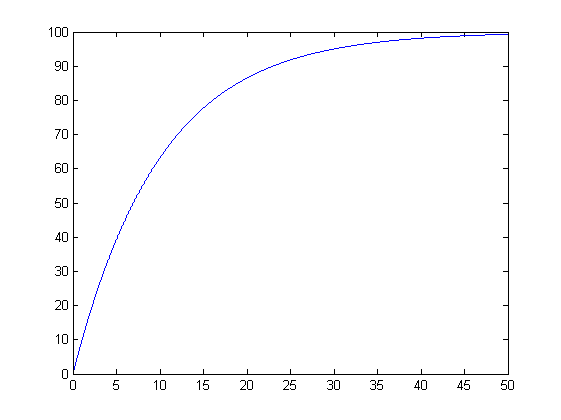
\includegraphics[width=0.5\textwidth]{mshape.png}
\caption{The shape of the Goel-Okumoto  }
\label{goelokumoto}
\end{figure}

\noindent By inserting the the value of $m(t_{i})$ for all $i$ into the likelihood function for the general NHPP model, and then maximising the likelihood function, the model parameters $a$ and $b$ can be estimated. 

\subsection{The Jelinski-Moranda model}
Time between failure models aim to model times between occurred failures. The Jelinski-Moranda model assumes that the times between failures are independently exponentially distributed according to 

$$\lambda_{i}=\phi(N-(i-1))$$

\noindent where $\lambda_{i}$ is assumed to be a function of the remaining number of failures, $N$ is the initial number of faults in the program and $\phi$ is a constant. 

The Jelinski-Moranda model describes a simplification of the real behavior where $N$ and $\phi$ are estimated from the measured data with, e.g., maximum likelihood estimation. 